\documentclass[10pt,a4paper]{amsart}
\usepackage[margin=19mm]{geometry}
\usepackage{amsmath,amssymb,mathtools}
\usepackage[scr=rsfs,cal=euler]{mathalfa}
\usepackage{xfrac}
\usepackage[unicode,hidelinks,bookmarks=false]{hyperref}
\newcommand{\ie}{i.e.\ }
\newcommand{\cf}{cf.\ }
\newcommand{\resp}{respectively\ }
\newcommand{\Subsection}{\subsection}
\providecommand{\nobreakdash}{\nobreak\hbox{-}}
\setlength{\emergencystretch}{2em}
\multlinegap0pt
\usepackage{tikz}
\usepackage{float}
\usepackage{amssymb}
\usepackage{mathtools}
\usepackage{bm}
\usepackage{xcolor}
\usepackage[shortlabels]{enumitem}
\usepackage[normalem]{ulem}
\usepackage{xfrac}
\newtheorem{lemma}{Lemma}
\title{Unimodality and Cluster Algebras from Surfaces}
\author{Wonwoo Kang, Kyeongjun Lee, Eunsung Lim}
\date{Source: arXiv:2508.04396v3 (CC BY 4.0)}
\begin{document}
\maketitle

\noindent\emph{Source and licence.} Unimodality and Cluster Algebras from Surfaces. Version arXiv:2508.04396v3 (CC BY 4.0), distributed by arXiv under the Creative Commons Attribution 4.0 International licence, http://creativecommons.org/licenses/by/4.0/, as recorded in the arXiv licence metadata for this exact version and shown on the abstract page https://arxiv.org/abs/2508.04396v3. Full licence notice: \texttt{licenses/arxiv-2508.04396-CC-BY-4.0.txt}.\par\smallskip

\noindent\textit{Editorial scope.} Counted unit: the article's lemma lem:eq1 (source0.tex lines 1026--1028). The article's complete original proof of it is delivered with it (source0.tex lines 1029--1199, one \texttt{proof} environment of 171 lines). No mathematics is written, repaired or re-derived: the statement and the proof are the article's own lines, in the article's own notation, and no retained line is substituted or re-flowed.  No further source-local context is needed: every cross-reference of every retained line resolves inside the two delivered spans.  Nothing was omitted from any retained span, so the package carries no omission record.  No retained line contains a citation, so the wrapper carries no bibliography and no bibliography entry.  The retained lines contain the article's own diagram code, which the wrapper typesets with the standard tikz packages; no image file is delivered and the package declares no asset dependency.  Editorial formatting only, in addition: an AMS \texttt{amsart} preamble that restates the article's own declarations and macros used by the retained lines, namely the environments \texttt{lemma} on separate counters, together with the standard packages those lines need.  The retained environments print in this document as Lemma 1 in order of appearance, whereas the article prints the same items with the numbering of its own full document.  The complete native source of the article as distributed in the arXiv e-print for this exact version is bundled unchanged as \texttt{sources/182800/source0.tex}.
\begin{lemma}\label{lem:eq1}
    The rank polynomial $R^{(n+1)}(\alpha; q)$ of the singly notched poset $P^{(n+1)}(\alpha)$ can be decomposed into the difference of two circular fence poset polynomials, weighted by a power of $q$, $q^{\alpha_s+1}$.
\end{lemma}

\begin{proof}
Let us consider the case when \( s \) is even. The case for odd \( s \) follows by simply exchanging each occurrence of \( v_n \) with \( v_{n - \alpha_s + 1} \).

Define \( P_T^{(n+1)}(\alpha) \) as the poset obtained by adding a new vertex \( v_T \) lying above both \( v_1 \) and \( v_{n - \alpha_s + 1} \) in the fence poset associated to \( \alpha \). Let \( R_T^{(n+1)}(\alpha; q) \) be the corresponding rank polynomial. The ideals of \( P_T^{(n+1)}(\alpha) \) are partitioned into those that include \( v_T \) and those that do not.

Let \( \beta \) be the composition obtained from \( \alpha \) by removing \( v_T \) and all vertices below it. Let \( d_1 \) denote the number of vertices below \( v_T \). Note that \( d_1 \geq \alpha_{s-1} + \alpha_s + 2 \), since \( v_T \) lies above every vertex \( v_i \) with \( n - \alpha_{s-1} - \alpha_s + 1 \leq i \leq n+1 \), and also above \( v_1 \). Then we have:
\[
R_T^{(n+1)}(\alpha; q) = R^{(n+1)}(\alpha; q) + q^{d_1 + 1} R(\beta; q).
\]

\begin{figure}[H]
    \centering
    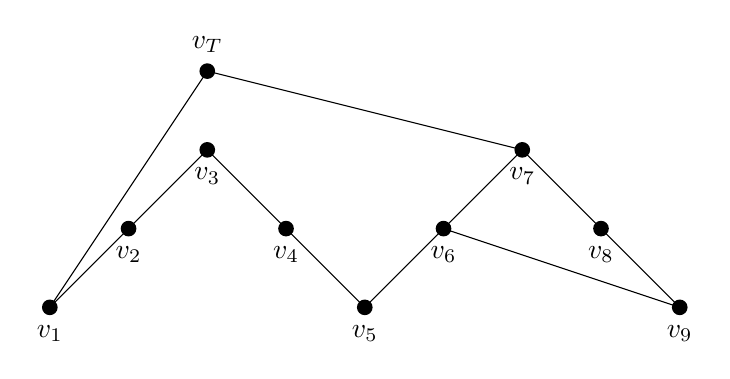
\begin{tikzpicture}
        \coordinate (x1) at (1, 2);
        \coordinate (x2) at (2, 3);
        \coordinate (x3) at (3, 4);
        \coordinate (x4) at (4, 3);
        \coordinate (x5) at (5, 2);
        \coordinate (x6) at (6, 3);
        \coordinate (x7) at (7, 4);
        \coordinate (x8) at (8, 3);
        \coordinate (x9) at (9, 2);
        \coordinate (xT) at (3, 5);

        \node[circle, fill=black, inner sep=2pt, label=below:$v_{1}$] at (x1) {};
        \node[circle, fill=black, inner sep=2pt, label=below:$v_{2}$] at (x2) {};
        \node[circle, fill=black, inner sep=2pt, label=below:$v_{3}$] at (x3) {};
        \node[circle, fill=black, inner sep=2pt, label=below:$v_{4}$] at (x4) {};
        \node[circle, fill=black, inner sep=2pt, label=below:$v_{5}$] at (x5) {};
        \node[circle, fill=black, inner sep=2pt, label=below:$v_{6}$] at (x6) {};
        \node[circle, fill=black, inner sep=2pt, label=below:$v_{7}$] at (x7) {};
        \node[circle, fill=black, inner sep=2pt, label=below:$v_{8}$] at (x8) {};
        \node[circle, fill=black, inner sep=2pt, label=below:$v_{9}$] at (x9) {};
        \node[circle, fill=black, inner sep=2pt, label=above:$v_{T}$] at (xT) {};

        \draw (x1) -- (x3);
        \draw (x3) -- (x5);
        \draw (x5) -- (x7);
        \draw (x7) -- (x9);
        \draw (x6) -- (x9);
        \draw (x1) -- (xT);
        \draw (x7) -- (xT);
    \end{tikzpicture}
    \caption{An example of \( P_T^{(n+1)}(\alpha) \) when \( \alpha = (2,2,2,2) \)}
    \label{fig:PT}
\end{figure}

Next, let \( \overline{P_T}(\alpha) \) be the circular poset obtained by removing the relation \( v_{n - \alpha_s} \prec v_{n - \alpha_s + 1} \) from \( P_T^{(n+1)}(\alpha) \), and let \( \overline{R_T}(\alpha; q) \) denote its rank polynomial.

Let \( \gamma \) be the poset obtained from \( \overline{P_T}(\alpha) \) by removing \( v_{n-\alpha_s} \) and all the vertices above it and removing \( v_{n - \alpha_s + 1} \) along with all the vertices below it. The ideals of \( \overline{P_T}(\alpha) \) then consist of:
(1) those in \( P_T^{(n+1)}(\alpha) \) and
(2) additional ideals of \( \gamma \), which correspond to including \( v_{n - \alpha_s + 1} \) but not \( v_{n - \alpha_s} \), weighted by \( q^{\alpha_s + 1} \).

Thus, we have the following.
\[
\overline{R_T}(\alpha; q) = R_T^{(n+1)}(\alpha; q) + q^{\alpha_s + 1} R(\gamma; q),
\]
which implies
\[
R^{(n+1)}(\alpha; q) = \overline{R_T}(\alpha; q) - q^{d_1 + 1} R(\beta; q) - q^{\alpha_s + 1} R(\gamma; q).
\]

Now, define the poset \( \delta \) as follows. Let \( \beta \cup \gamma \) be the union of the underlying sets of \( \beta \) and \( \gamma \), preserving their partial orders. \( v_T \) will be one endpoint of $\beta\cup \gamma$ and let the other vertex as \( v_P \) where \( 1 \leq P \leq n - \alpha_s - 1 \). To extend this structure, we introduce an additional vertex $v_{P+1}$ and prescribe a relation between $v_P$ and $v_{P+1}$ consistent with the composition $\alpha$. Finally, we impose the additional relation $v_T \prec v_{P+1}$ and relabel $v_{P+1}$ as $v_{\tilde{T}}$. The resulting structure constitutes the circular fence poset $\delta$.

\begin{table}[htbp]
    \centering
    \begin{tabular}{|c|c|c|}
    \hline
           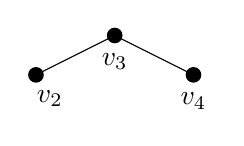
\begin{tikzpicture}
        \coordinate (x2) at (2, .5);
        \coordinate (x3) at (3, 1);
        \coordinate (x4) at (4, .5);

        \node[circle, fill=black, inner sep=2pt, label={[below,xshift=5pt,yshift=-5pt]{$v_{2}$}}] (nodex2) at (x2) {};
        \node[circle, fill=black, inner sep=2pt, label=below:$v_{3}$] (nodex3) at (x3) {};
        \node[circle, fill=black, inner sep=2pt, label=below:$v_{4}$] (nodex4) at (x4) {};

        \draw[-] (x2) -- (x3);
        \draw[-] (x3) -- (x4);
    \end{tikzpicture}
  & 
      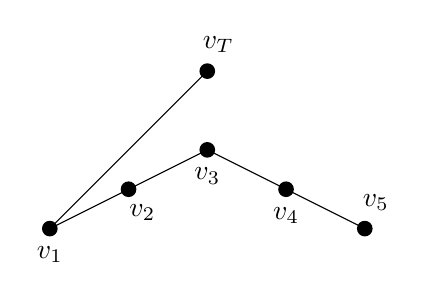
\begin{tikzpicture}
        \coordinate (x1) at (1, 0);
        \coordinate (x2) at (2, .5);
        \coordinate (x3) at (3, 1);
        \coordinate (x4) at (4, .5);
        \coordinate (x5) at (5, 0);
        \coordinate (xT) at (3, 2);

        \node[circle, fill=black, inner sep=2pt, label=below:$v_{1}$] (nodex1) at (x1) {};
        \node[circle, fill=black, inner sep=2pt, label={[below,xshift=5pt,yshift=-5pt]{$v_{2}$}}] (nodex2) at (x2) {};
        \node[circle, fill=black, inner sep=2pt, label=below:$v_{3}$] (nodex3) at (x3) {};
        \node[circle, fill=black, inner sep=2pt, label=below:$v_{4}$] (nodex4) at (x4) {};
        \node[circle, fill=black, inner sep=2pt, label={[above,xshift=4pt]{$v_{5}$}}] (nodex5) at (x5) {};
        \node[circle, fill=black, inner sep=2pt, label={[above,xshift=4pt]{$v_{T}$}}] (nodexT) at (xT) {};

        \draw[-] (x1) -- (x3);
        \draw[-] (x3) -- (x5);
        \draw[-] (x1) -- (xT);
    \end{tikzpicture}

&    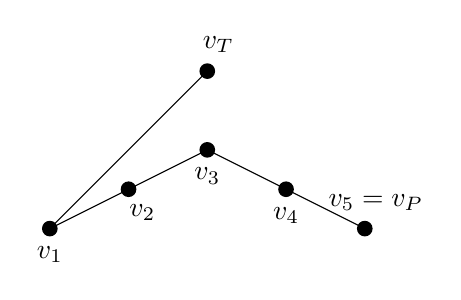
\begin{tikzpicture}
        \coordinate (x1) at (1, 0);
        \coordinate (x2) at (2, .5);
        \coordinate (x3) at (3, 1);
        \coordinate (x4) at (4, .5);
        \coordinate (x5) at (5, 0);
        \coordinate (xT) at (3, 2);

        \node[circle, fill=black, inner sep=2pt, label=below:$v_{1}$] (nodex1) at (x1) {};
        \node[circle, fill=black, inner sep=2pt, label={[below,xshift=5pt,yshift=-5pt]{$v_{2}$}}] (nodex2) at (x2) {};
        \node[circle, fill=black, inner sep=2pt, label=below:$v_{3}$] (nodex3) at (x3) {};
        \node[circle, fill=black, inner sep=2pt, label=below:$v_{4}$] (nodex4) at (x4) {};
        \node[circle, fill=black, inner sep=2pt, label={[above,xshift=4pt]{$v_{5}=v_P$}}] (nodex5) at (x5) {};
        \node[circle, fill=black, inner sep=2pt, label={[above,xshift=4pt]{$v_{T}$}}] (nodexT) at (xT) {};

        \draw[-] (x1) -- (x3);
        \draw[-] (x3) -- (x5);
        \draw[-] (x1) -- (xT);
    \end{tikzpicture}\\
    \hline
    $\beta$& $\gamma$ & $\beta\cup\gamma$\\
    \hline
    \end{tabular}
    \caption{$\beta$, $\gamma$, and $\beta\cup\gamma$ for $P^{(n+1)}_T(\alpha)$ when $\alpha=(2,2,2,2)$}
    \label{tab:topex}
\end{table}

\begin{figure}[H]
    \centering
    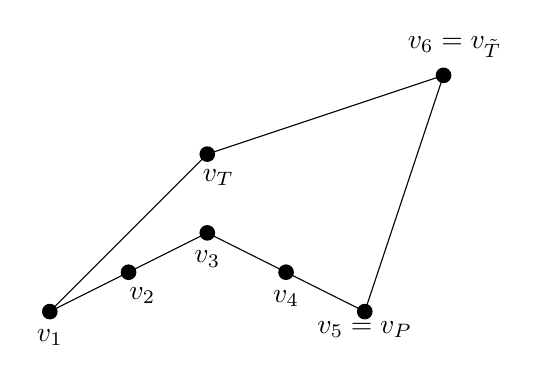
\begin{tikzpicture}
        \coordinate (x1) at (1, 0);
        \coordinate (x2) at (2, .5);
        \coordinate (x3) at (3, 1);
        \coordinate (x4) at (4, .5);
        \coordinate (x5) at (5, 0);
        \coordinate (xT) at (3, 2);
        \coordinate (xT') at (6, 3);


        \node[circle, fill=black, inner sep=2pt, label=below:$v_{1}$] (nodex1) at (x1) {};
        \node[circle, fill=black, inner sep=2pt, label={[below,xshift=5pt,yshift=-5pt]{$v_{2}$}}] (nodex2) at (x2) {};
        \node[circle, fill=black, inner sep=2pt, label=below:$v_{3}$] (nodex3) at (x3) {};
        \node[circle, fill=black, inner sep=2pt, label=below:$v_{4}$] (nodex4) at (x4) {};
        \node[circle, fill=black, inner sep=2pt, label={[below,yshift=-3pt]{$v_{5}=v_P$}}] (nodex5) at (x5) {};
        \node[circle, fill=black, inner sep=2pt, label={[below,xshift=4pt,yshift=-5pt]{$v_{T}$}}] (nodexT) at (xT) {};
        \node[circle, fill=black, inner sep=2pt, label={[above,xshift=4pt]{$v_6=v_{\tilde{T}}$}}] (nodexT') at (xT') {};

        \draw[-] (x1) -- (x3);
        \draw[-] (x3) -- (x5);
        \draw[-] (x5) -- (xT');
        \draw[-] (x1) -- (xT);
        \draw[-] (xT) -- (xT');
    \end{tikzpicture}
    \caption{$\delta$ for $P^{(n+1)}_T(\alpha)$ when $\alpha=(2,2,2,2)$}
    \label{fig:delta}
\end{figure}

There are now two types of ideals in \( \delta \):
- those that include \( v_{\tilde{T}} \), contributing \( q^{d_1 - \alpha_s} R(\beta; q) \), - and those that exclude it, contributing \( R(\gamma; q) \).

Thus, we obtain:
\[
\overline{R}(\delta; q) = q^{d_1 - \alpha_s} R(\beta; q) + R(\gamma; q).
\]

Substituting into the earlier expression gives:
\begin{align}\label{eq:1}
R^{(n+1)}(\alpha; q) = \overline{R_T}(\alpha; q) - q^{\alpha_s+ 1} \overline{R}(\delta; q).
\end{align}
\end{proof}

\end{document}
